
\documentclass[aspectratio=169,11pt]{beamer}

\usetheme{Madrid}
\usecolortheme{default}

\usepackage{amsmath,amssymb}
\usepackage{booktabs}
\usepackage{tikz}
\usepackage{pgfplots}
\pgfplotsset{compat=1.18}

\definecolor{navy}{RGB}{22,47,81}
\definecolor{teal}{RGB}{0,130,120}

\setbeamercolor{structure}{fg=navy}
\setbeamercolor{frametitle}{
    fg=white,bg=navy
}
\setbeamercolor{title}{
    fg=white,bg=navy
}

\setbeamertemplate{navigation symbols}{}
\setbeamertemplate{footline}[frame number]

\title[NeuroRank 2.0]{
NeuroRank 2.0
}

\subtitle{
Retrieval-Aware Learning-to-Rank
and Query-Dependent Model Selection
for E-Commerce Search
}

\author{Bhukya Kasi}

\institute{
Indian Institute of Technology Dharwad
}

\date{October 2026}

\begin{document}

% ------------------------------------------------
\begin{frame}
\titlepage
\end{frame}

% ------------------------------------------------
\begin{frame}{Research Motivation}

\textbf{Problem:}
Product search must identify relevant
items from a large catalog.

\vspace{0.4cm}

\begin{itemize}
\item Lexical retrieval relies on
matching words.

\item Dense retrieval captures
semantic relationships.

\item Learning-to-rank can combine
multiple relevance features.

\item However, training candidates
may differ from candidates retrieved
during inference.
\end{itemize}

\vspace{0.3cm}

\begin{block}{Research Question}
Do supervised and query-dependent
ranking strategies improve
end-to-end search performance
under retrieval-generated
candidate distributions?
\end{block}

\end{frame}

% ------------------------------------------------
\begin{frame}{Project Objectives}

\begin{enumerate}
\item Build a working hybrid product
retrieval system.

\item Integrate BM25, MiniLM
embeddings, and FAISS.

\item Train a retrieval-aware
LambdaMART ranking model.

\item Develop an experimental
query-dependent adaptive selector.

\item Compare methods using
held-out relevance judgments.

\item Provide reproducible API
and interactive dashboard.
\end{enumerate}

\end{frame}

% ------------------------------------------------
\begin{frame}{NeuroRank Architecture}

\centering

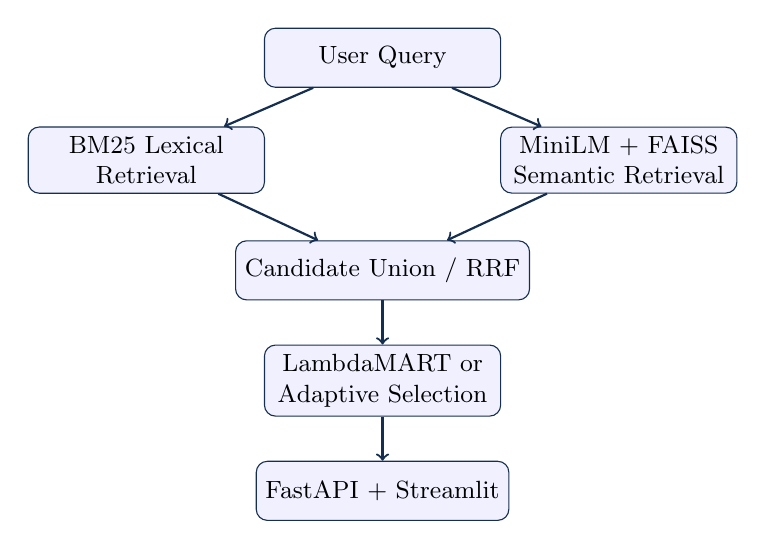
\begin{tikzpicture}[
node distance=1.15cm,
every node/.style={font=\small},
box/.style={
draw=navy,
rounded corners,
fill=blue!6,
minimum width=3.0cm,
minimum height=0.75cm,
align=center
},
arrow/.style={
->,thick,navy
}
]

\node[box] (query) at (0,3.1)
{User Query};

\node[box] (bm25) at (-3,1.8)
{BM25 Lexical\\Retrieval};

\node[box] (minilm) at (3,1.8)
{MiniLM + FAISS\\Semantic Retrieval};

\node[box] (fusion) at (0,0.4)
{Candidate Union / RRF};

\node[box] (rank) at (0,-1.0)
{LambdaMART or\\Adaptive Selection};

\node[box] (api) at (0,-2.4)
{FastAPI + Streamlit};

\draw[arrow] (query) -- (bm25);
\draw[arrow] (query) -- (minilm);
\draw[arrow] (bm25) -- (fusion);
\draw[arrow] (minilm) -- (fusion);
\draw[arrow] (fusion) -- (rank);
\draw[arrow] (rank) -- (api);

\end{tikzpicture}

\end{frame}

% ------------------------------------------------
\begin{frame}{Lexical and Semantic Retrieval}

\textbf{BM25:}

\[
s_B(q,d)=
\sum_{t\in q}
\mathrm{IDF}(t)
\frac{
f(t,d)(k_1+1)
}{
f(t,d)+
k_1
\left(
1-b+b\frac{|d|}{\mathrm{avgdl}}
\right)
}
\]

\vspace{0.3cm}

\textbf{MiniLM:}

\[
s_S(q,d)=
\frac{
f_\theta(q)^\top f_\theta(d)
}{
\|f_\theta(q)\|
\|f_\theta(d)\|
}
\]

\begin{itemize}
\item BM25 measures lexical
term relevance.
\item MiniLM measures dense
semantic similarity.
\item FAISS retrieves products
using vector inner products.
\end{itemize}

\end{frame}

% ------------------------------------------------
\begin{frame}{Candidate Fusion}

Two retrievers each return
up to 100 candidates.

\[
\mathcal{C}(q)=
\mathcal{C}_{B}(q)
\cup
\mathcal{C}_{S}(q)
\]

Maximum candidate-pool size:
200 unique products.

\vspace{0.4cm}

\textbf{Reciprocal Rank Fusion:}

\[
s_{\mathrm{RRF}}(d)=
\sum_{r\in\{B,S\}}
\frac{
\mathbf{1}[d\in\mathcal{C}_r]
}{
60+\mathrm{rank}_r(d)
}
\]

\vspace{0.2cm}

RRF combines rank positions
without requiring comparable
raw BM25 and MiniLM scores.

\end{frame}

% ------------------------------------------------
\begin{frame}{LambdaMART Reranking}

The supervised ranker uses
eight features:

\begin{columns}

\column{0.52\textwidth}

\begin{itemize}
\item BM25 score
\item Semantic similarity
\item Query-title overlap
\item Exact phrase match
\item BM25 reciprocal rank
\item Semantic reciprocal rank
\item Title length
\item Query length
\end{itemize}

\column{0.48\textwidth}

\[
\mathbf{x}\in\mathbb{R}^{8}
\]

\[
s_L(q,d)=
F_{\mathrm{LGBM}}(\mathbf{x})
\]

\vspace{0.25cm}

\textbf{ESCI label gains:}

\[
I=0,\quad C=1
\]

\[
S=3,\quad E=7
\]

\end{columns}

\end{frame}

% ------------------------------------------------
\begin{frame}{Adaptive Model Selection}

\textbf{Hypothesis:}
Different ranking models may perform
better on different query types.

\vspace{0.3cm}

The selector uses query-text features:

\begin{itemize}
\item Word count and character count
\item Lexical diversity
\item Average token length
\item Tokens containing digits
\end{itemize}

\[
p(q)=P(L>S\mid\mathbf{z}(q))
\]

\[
\mathrm{Method}(q)=
\begin{cases}
\mathrm{LambdaMART},&p(q)>0.5\\
\mathrm{MiniLM},&\text{otherwise}
\end{cases}
\]

\begin{alertblock}{Scope}
Experimental query-dependent selector;
not a calibrated uncertainty model.
\end{alertblock}

\end{frame}

% ------------------------------------------------
\begin{frame}{Experimental Dataset}

\begin{columns}

\column{0.50\textwidth}

\textbf{Amazon ESCI}

\begin{itemize}
\item Exact (E)
\item Substitute (S)
\item Complement (C)
\item Irrelevant (I)
\end{itemize}

\vspace{0.3cm}

\textbf{Research catalog:}

13,083 products

\column{0.50\textwidth}

\textbf{Query-disjoint splits}

\begin{tabular}{lr}
\toprule
Split & Queries\\
\midrule
Training & 400\\
Validation & 100\\
Held-out test & 100\\
\bottomrule
\end{tabular}

\end{columns}

\vspace{0.4cm}

\begin{block}{Evaluation Policy}
Unjudged products are assigned zero gain
for end-to-end NDCG, but they are not
treated as verified negative examples
for supervised training.
\end{block}

\end{frame}

% ------------------------------------------------
\begin{frame}{Evaluation Metrics}

\textbf{Normalized Discounted
Cumulative Gain}

\[
\mathrm{DCG}@k=
\sum_{i=1}^{k}
\frac{2^{rel_i}-1}
{\log_2(i+1)}
\]

\[
\mathrm{NDCG}@k=
\frac{
\mathrm{DCG}@k
}{
\mathrm{IDCG}@k
}
\]

\vspace{0.35cm}

\textbf{Recall}

\[
\mathrm{Recall}@k=
\frac{
|\mathrm{Relevant}
\cap\mathrm{Top}_k|
}{
|\mathrm{Relevant}|
}
\]

\end{frame}

% ------------------------------------------------
\begin{frame}{Held-Out Experimental Results}

\centering

\begin{table}
\small
\begin{tabular}{lccc}
\toprule
Method &
NDCG@10 &
Recall@10 &
Recall@100\\
\midrule
BM25 &
0.4981 & 0.3589 & 0.6432\\
MiniLM &
0.5407 & 0.3965 & 0.7538\\
\textbf{RRF} &
\textbf{0.5445} &
\textbf{0.4018} &
\textbf{0.7682}\\
LambdaMART &
0.5088 & 0.3692 & 0.7536\\
Adaptive &
0.5325 & 0.3885 & 0.7549\\
\bottomrule
\end{tabular}
\end{table}

\vspace{0.35cm}

\begin{block}{Observed Result}
RRF achieved the highest
measured NDCG@10 and recall
on the 100 held-out queries.
\end{block}

\end{frame}

% ------------------------------------------------
\begin{frame}{Visual Comparison: NDCG@10}

\centering

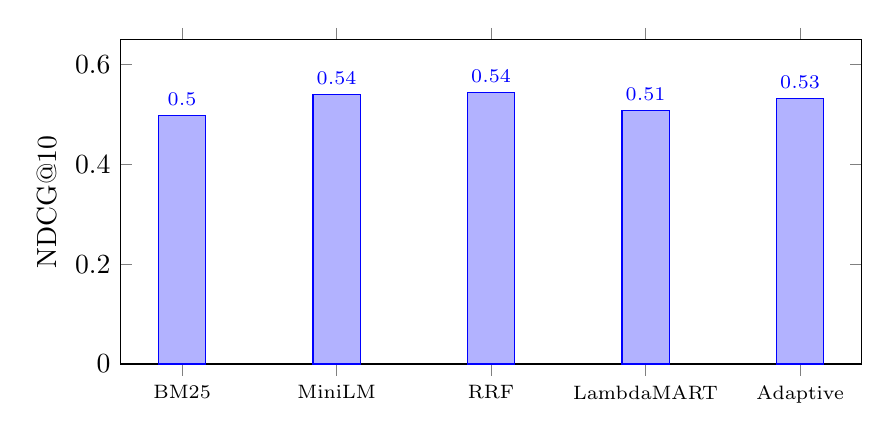
\begin{tikzpicture}

\begin{axis}[
ybar,
width=11cm,
height=5.7cm,
bar width=17pt,
ymin=0,
ymax=0.65,
ylabel={NDCG@10},
symbolic x coords={
BM25,MiniLM,RRF,LambdaMART,Adaptive
},
xtick=data,
x tick label style={
font=\scriptsize
},
nodes near coords,
nodes near coords style={
font=\scriptsize
},
every axis plot/.append style={
fill=teal,
draw=teal
}
]

\addplot coordinates {
(BM25,0.4981)
(MiniLM,0.5407)
(RRF,0.5445)
(LambdaMART,0.5088)
(Adaptive,0.5325)
};

\end{axis}
\end{tikzpicture}

\end{frame}

% ------------------------------------------------
\begin{frame}{Statistical Analysis}

\textbf{RRF versus MiniLM}

\[
\Delta\mathrm{NDCG}@10
\approx 0.00386
\]

95\% paired bootstrap interval:

\[
[-0.0327,\;0.0392]
\]

Holm-adjusted permutation test:

\[
p_{\mathrm{Holm}}=1.0
\]

\begin{alertblock}{Conclusion}
The observed RRF advantage over MiniLM
is not statistically established.
\end{alertblock}

\vspace{0.2cm}

\textbf{RRF versus BM25:}

\[
\Delta\approx0.0464,\qquad
CI_{95\%}\approx[0.0223,0.0724].
\]

\end{frame}

% ------------------------------------------------
\begin{frame}{Model Behavior and Limitations}

\textbf{Additional observations:}

\begin{itemize}
\item Candidate-pool recall:
approximately 79.46\%.

\item Adaptive selector chose
LambdaMART for 10 of
100 held-out queries.

\item Supervised and adaptive
ranking did not outperform
the strongest retrieval baselines.

\item The test evaluates unseen
queries within a fixed catalog.

\item Sparse judgments can
underestimate relevance
of retrieved products.
\end{itemize}
